\section{MEWE}
\label{section:mewe}

\newcommand{\tool}{MEWE\xspace}
\newcommand{\repourl}{TODO}
% Overview
This section describes MEWE, our second contribution. 
%MEWE is implemented in 942 lines of C++ code.
The core idea of \tool is to synthesize diversified function variants, using CROW, providing execution-path randomization in an MVE. Thus, the goal of \tool is to synthesize multivariant  \wasm binaries. %, according to the threat model presented in \autoref{sec:threat-model}. 
The tool generates application-level multivariant binaries, without any change to the operating system or \wasm runtime.
%It uses the LLVM 12.0.0 libraries to extend the LLVM standard linker tool capability with the multivariant generation.
%Per Crane et al. the execution-path randomization is made to hinder side-channel attacks \cite{crane2015thwarting}. 
% All programs are diversified with behavior preservation guarantees according to the design of CROW (\autoref{section:crow}).
MEWE creates an MVE by intermixing functions for which CROW generates variants.
CROW generates each one of these variants with fine-grained diversification at instruction level, applying the majority of the strategies discussed in \autoref{sota:sota} and \emph{constant inferring}. Besides, \tool inlines function variants when appropriate, also resulting in call stack diversification at runtime.

In \autoref{workflow}, we summarize the analysis and transformation pipeline of \tool.
We pass a bitcode to be diversified, as an input to \tool.
% Move this to the previous section
%LLVM binaries can be obtained from any language with an LLVM frontend such as C/C++, Rust or Go, and they can easily be compiled to WebAssembly.
In Step~\step{1}, the binary is passed to CROW. 
Step~\step{2} packages all the variants in one single multivariant LLVM binary. 
In Step~\step{3}, we use a special component, called a ``mixer``,  which augments the binary with a random generator, which is required for performing the execution-path randomization. 
Also at this stage, the multivariant binary is fixed with the entrypoint of the original binary.
%The harness is used to connect the program to its original execution environment while the generator provides support for random execution path at runtime.
The final output of Step~\step{4} is a standalone multivariant \wasm binary that can be directly deployed. 
The source code of MEWE can be found at \todo{}.

%For sake of open science and for fostering research on this important topic, the code of \tool is made publicly available on GitHub: \repourl.

\begin{figure*}
  \centering
  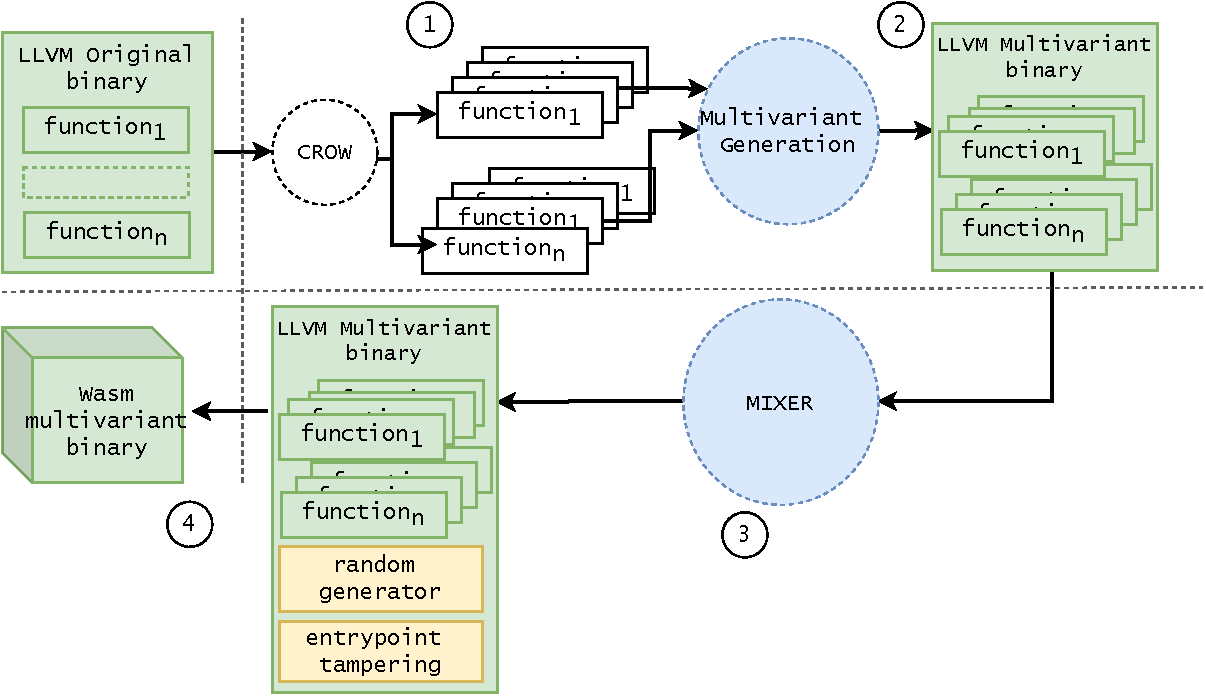
\includegraphics[width=\linewidth]{diagrams/MEWE.pdf}
  \caption{Overview of \tool. It takes as input an LLVM binary. It first generates a set of functionally equivalent variants for each function in the binary and then generates a LLVM multivariant binary composed of all the function variants. Also, it includes the dispatcher functions in charge of selecting a variant when a function is invoked. The \tool mixer composes the LLVM multivariant binary with a random number generation library and a tampering of the original application entrypoint, in order to produce a \wasm multivariant binary ready to be deployed. }
  \label{workflow}
\end{figure*}

\begin{comment}

%\subsection{Variant generation}

% How CROW works ?
%\tool relies on the superdiversifier CROW \cite{CabreraArteaga2020CROWCD} to automatically diversify each function in the input LLVM binary (Step~\step{1}). CROW receives an LLVM module, analyzes the binary at the function block level and generates semantically equivalent variants for each function, if they exist. CROW variants are verified as semantically equivalent with an SMT solver. 
%Here, we define a function variant as:

%\begin{definition}{Function variant:}\label{def:variant}
%    Let $F$ be a function, $F'$ is a function variant of $F$ for \tool if it is semantically equivalent  (i.e., same input/output behavior), but exhibits a different internal behavior through tracing. 
%\end{definition}

%In \autoref{example:eq_code}, we illustrate two semantically equivalent Wasm functions according to \autoref{def:variant}. 
%The left most listing corresponds to the Wasm module shown in \autoref{WasmExample}.
%The right most listing is a variant for this function.
%We can appreciate that the multiplication of the original code, in the third and four lines, is replaced by an addition, making the variant to have the same semantic but executing different instructions.
\lstset{
    language=WAT,
    style=WATStyle,
    stepnumber=0,
    label=EQExample}
\begin{minipage}{0.9\linewidth}
    \begin{minipage}{0.4\linewidth}
        \begin{lstlisting}
...
(func (;0;)
    local.get 0
    local.get 0
    i32.const 2
    i32.mul
    i32.add)
...
        \end{lstlisting}
    \end{minipage}
        \begin{minipage}{0.45\linewidth}
        \begin{lstlisting}
...
(func (;0;)
    local.get 0
    local.get 0
    local.get 0
    i32.add
    i32.add)
...
        \end{lstlisting}
    \end{minipage}
    \noindent\rule{\linewidth}{0.4pt}
    \captionof{lstlisting}{Example of two semantically equivalent functions. The left listing corresponds to the original code. The right listing shows a semantically equivalent variant.}\label{example:eq_code}

\end{minipage}

\vspace{2mm}

CROW synthesizes variants by enumerative synthesis based on code transformation. 
The most relevant transformations are: constant inferring to replace control flow statements, arithmetic's equivalent replacement, and loop unrolling. 
CROW performs stacked transformations, this means that it can synthesize variants of different size, i.e., from smaller to larger variants than the original.

% Soundness
The variants created by CROW are artificially synthesized from the original binary. 
CROW checks for semantic equivalence of both codes, original and variant using the symbolic execution.
If the behavior of the variant is not the reference behavior, the variant is discarded.
This means that, after Step \step{1}, the variant is necessarily equivalent to the original program.


\end{comment}

\subsection*{Combining variants into multivariant functions}

The key component of \tool consists in combining the variants generated for the original functions, into a single binary.
The goal is to support execution-path randomization at runtime.
% General idea
The core idea is to introduce one dispatcher function per original function for which we generate variants.
A dispatcher function is a synthetic function that is in charge of choosing a variant at random, every time the original function is invoked during the execution.
With the introduction of dispatcher function,  \tool turns the original call graph into a multivariant call graph, defined as follows. 

\begin{definition}{Multivariant Call Graph (MCG):}\label{def:EP}
    A multivariant call graph is a call graph $\langle N,E \rangle$ where the nodes in $N$ represent all the functions in the binary and an edge $(f_1,f_2) \in E$ represents a possible invocation of $f_2$ by $f_1$  \cite{ryder1979}, where the nodes are typed. The nodes in $N$ have three possible types: a function present in the original program,  a generated function variant, or a dispatcher function.
\end{definition}


\begin{figure}
    \centering
  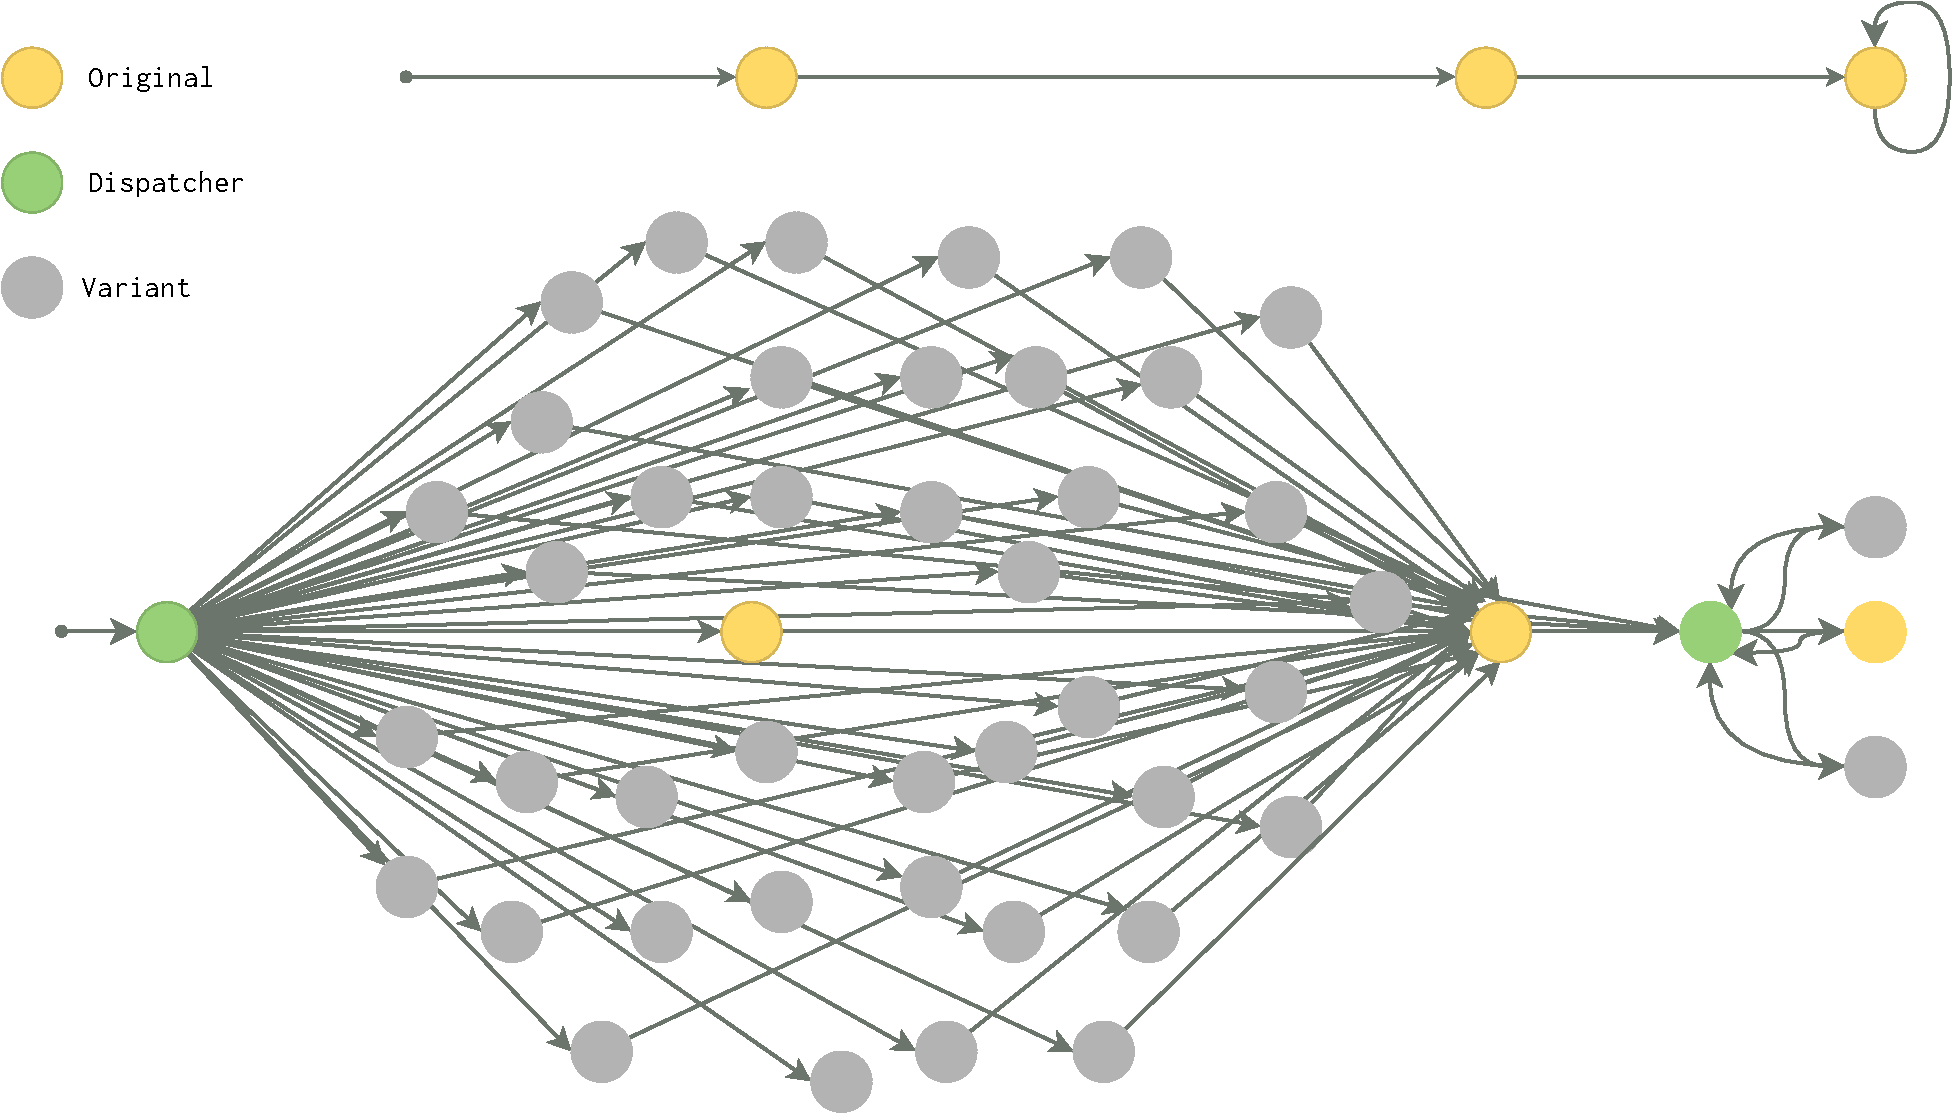
\includegraphics[width=.8\linewidth]{diagrams/CFG.pdf}
  \caption{Example of two static call graphs. At the top, the original call graph, at the bottom, the multivariant call graph, which includes nodes that represent function variants (in grey), dispatchers (in green), and original functions  (in yellow).
}
  \label{multivariant}
\end{figure}

% Instance of a multivariant module
In \autoref{multivariant}, we show the original static call graph for and original program (top of the figure), as well as the multivariant call graph generated with \tool (bottom of the figure).
The grey nodes represent function variants, the green nodes function dispatchers and the yellow nodes are the original functions.
The possible calls are represented by the directed edges.
The original program includes 3 functions. \tool generates 43 variants for the first function, none for the second and three for the third function. 
\tool introduces two dispatcher nodes, for the first and third functions. Each dispatcher is connected to the corresponding function variants, in order to invoke one variant randomly at runtime.


% exaplanation of dispatcher
In  \autoref{listing:multivariant_template}, we illustrate the LLVM construction for the function dispatcher corresponding to the right most green node of \autoref{multivariant}.
% General logic of a multivartiant function
It first calls the random generator, which returns a value that is then used to invoke a specific function variant. It should be noted that the dispatcher function is constructed using the same signature as the original function. 


\lstset{
    language=llvm,
    %style=nccode,
    basicstyle=\footnotesize\ttfamily,
    columns=fullflexible,
    breaklines=true,
    numbers=none,
    stepnumber=1,
    float
}

\begin{code}
\scriptsize
\noindent\begin{minipage}[b]{\linewidth}
    \begin{minipage}[t]{1\linewidth}
        \begin{lstlisting}[escapeinside={(*}{*)}]
define internal i32 @foo(i32 %0) {
    entry:
      %1 = call i32 @discriminate(i32 3)
      switch i32 %1, label %end [
        i32 0, label %case_43_
        i32 1, label %case_44_
      ]
    case_43_:                 
      %2 = call i32 @foo_43_(%0)
      ret i32 %2
    case_44_:                
      %3 = <body of foo_44_ inlined>
      ret i32 %3
    end:                                             
      %4 = call i32 @foo_original(%0)
      ret i32 %4
}
        \end{lstlisting}
    \end{minipage}%
    
    \noindent\rule{\linewidth}{0.4pt}
    \captionof{lstlisting}{Dispatcher function embedded in the multivariant binary of the original function in the rightmost green node in \autoref{multivariant}.}\label{listing:multivariant_template}
\end{minipage}
\end{code}

% Why a linear based switch
We implement the dispatchers with a switch-case structure to avoid indirect calls that can be susceptible to speculative execution based attacks \cite{Narayan2021Swivel}. 
The choice of a switch-case also avoids having multiple function definitions with the same signature, which could increase the attack surface in case the function signature is vulnerable \cite{johnson2021}.
This also allows \tool to inline function variants inside the dispatcher, instead of defining them again.
Here we trade security over performance, since dispatcher functions  that perform indirect calls, instead of a switch-case,  could improve the performance  of the dispatchers as indirect calls have constant time.

\begin{comment}

\subsection*{MEWE's Mixer}

The \tool mixer has four specific objectives: tamper the entrypoint of the application, link the LLVM multivariant binary, inject a random generator and merge all these components into a multivariant \wasm binary.
% Implementation
We use the Rustc compiler\footnote{\url{https://doc.rust-lang.org/rustc/what-is-rustc.html}} to orchestrate the mixing.
% The random number generation
For the random generator, we rely on WASI's specification \cite{WASI} for the random behavior of the dispatchers. Its exact implementation is dependent on the platform on which the binary is deployed.

The \tool mixer creates a new entrypoint for the binary called \emph{entrypoint tampering}.
It simply wraps the dispatcher for the entrypoint variants as a new function for the final Wasm binary and is declared as the application entrypoint. %This fixes an issue with  

\end{comment}
% How to turn function into endpoints
%The entrypoint tampering is needed for binariess passed to MEWE. We refer to the entrypoint as the entering main function of the original binary passed to MEWE. The tampering is needed because dispatchers for entrypoint variants make the multivariant invalid to be directly executed after it is compiled to Wasm.

%Throughout this paper, we refer to an endpoint as the closure of invoked functions when the entry point of the \wasm binary is executed.



\begin{comment}

\subsection{Multivariant Binary Execution at the Edge}

\todo{Introduce as the use of MEWE}

% What really is executed is the x86 code
When a WebAssembly binary is deployed on an edge platform, it is translated to machine code on the fly.
For our experiment, we deploy on the production edge nodes of Fastly. This edge computing platform uses Lucet, a native WebAssembly compiler and runtime, to compile and run the deployed Wasm binary \footnote{\url{https://github.com/bytecodealliance/lucet}}.
Lucet generates x86 machine code and ensures that the generated machine code executes inside a secure sandbox, controlling memory isolation.


\begin{figure}
\centering
  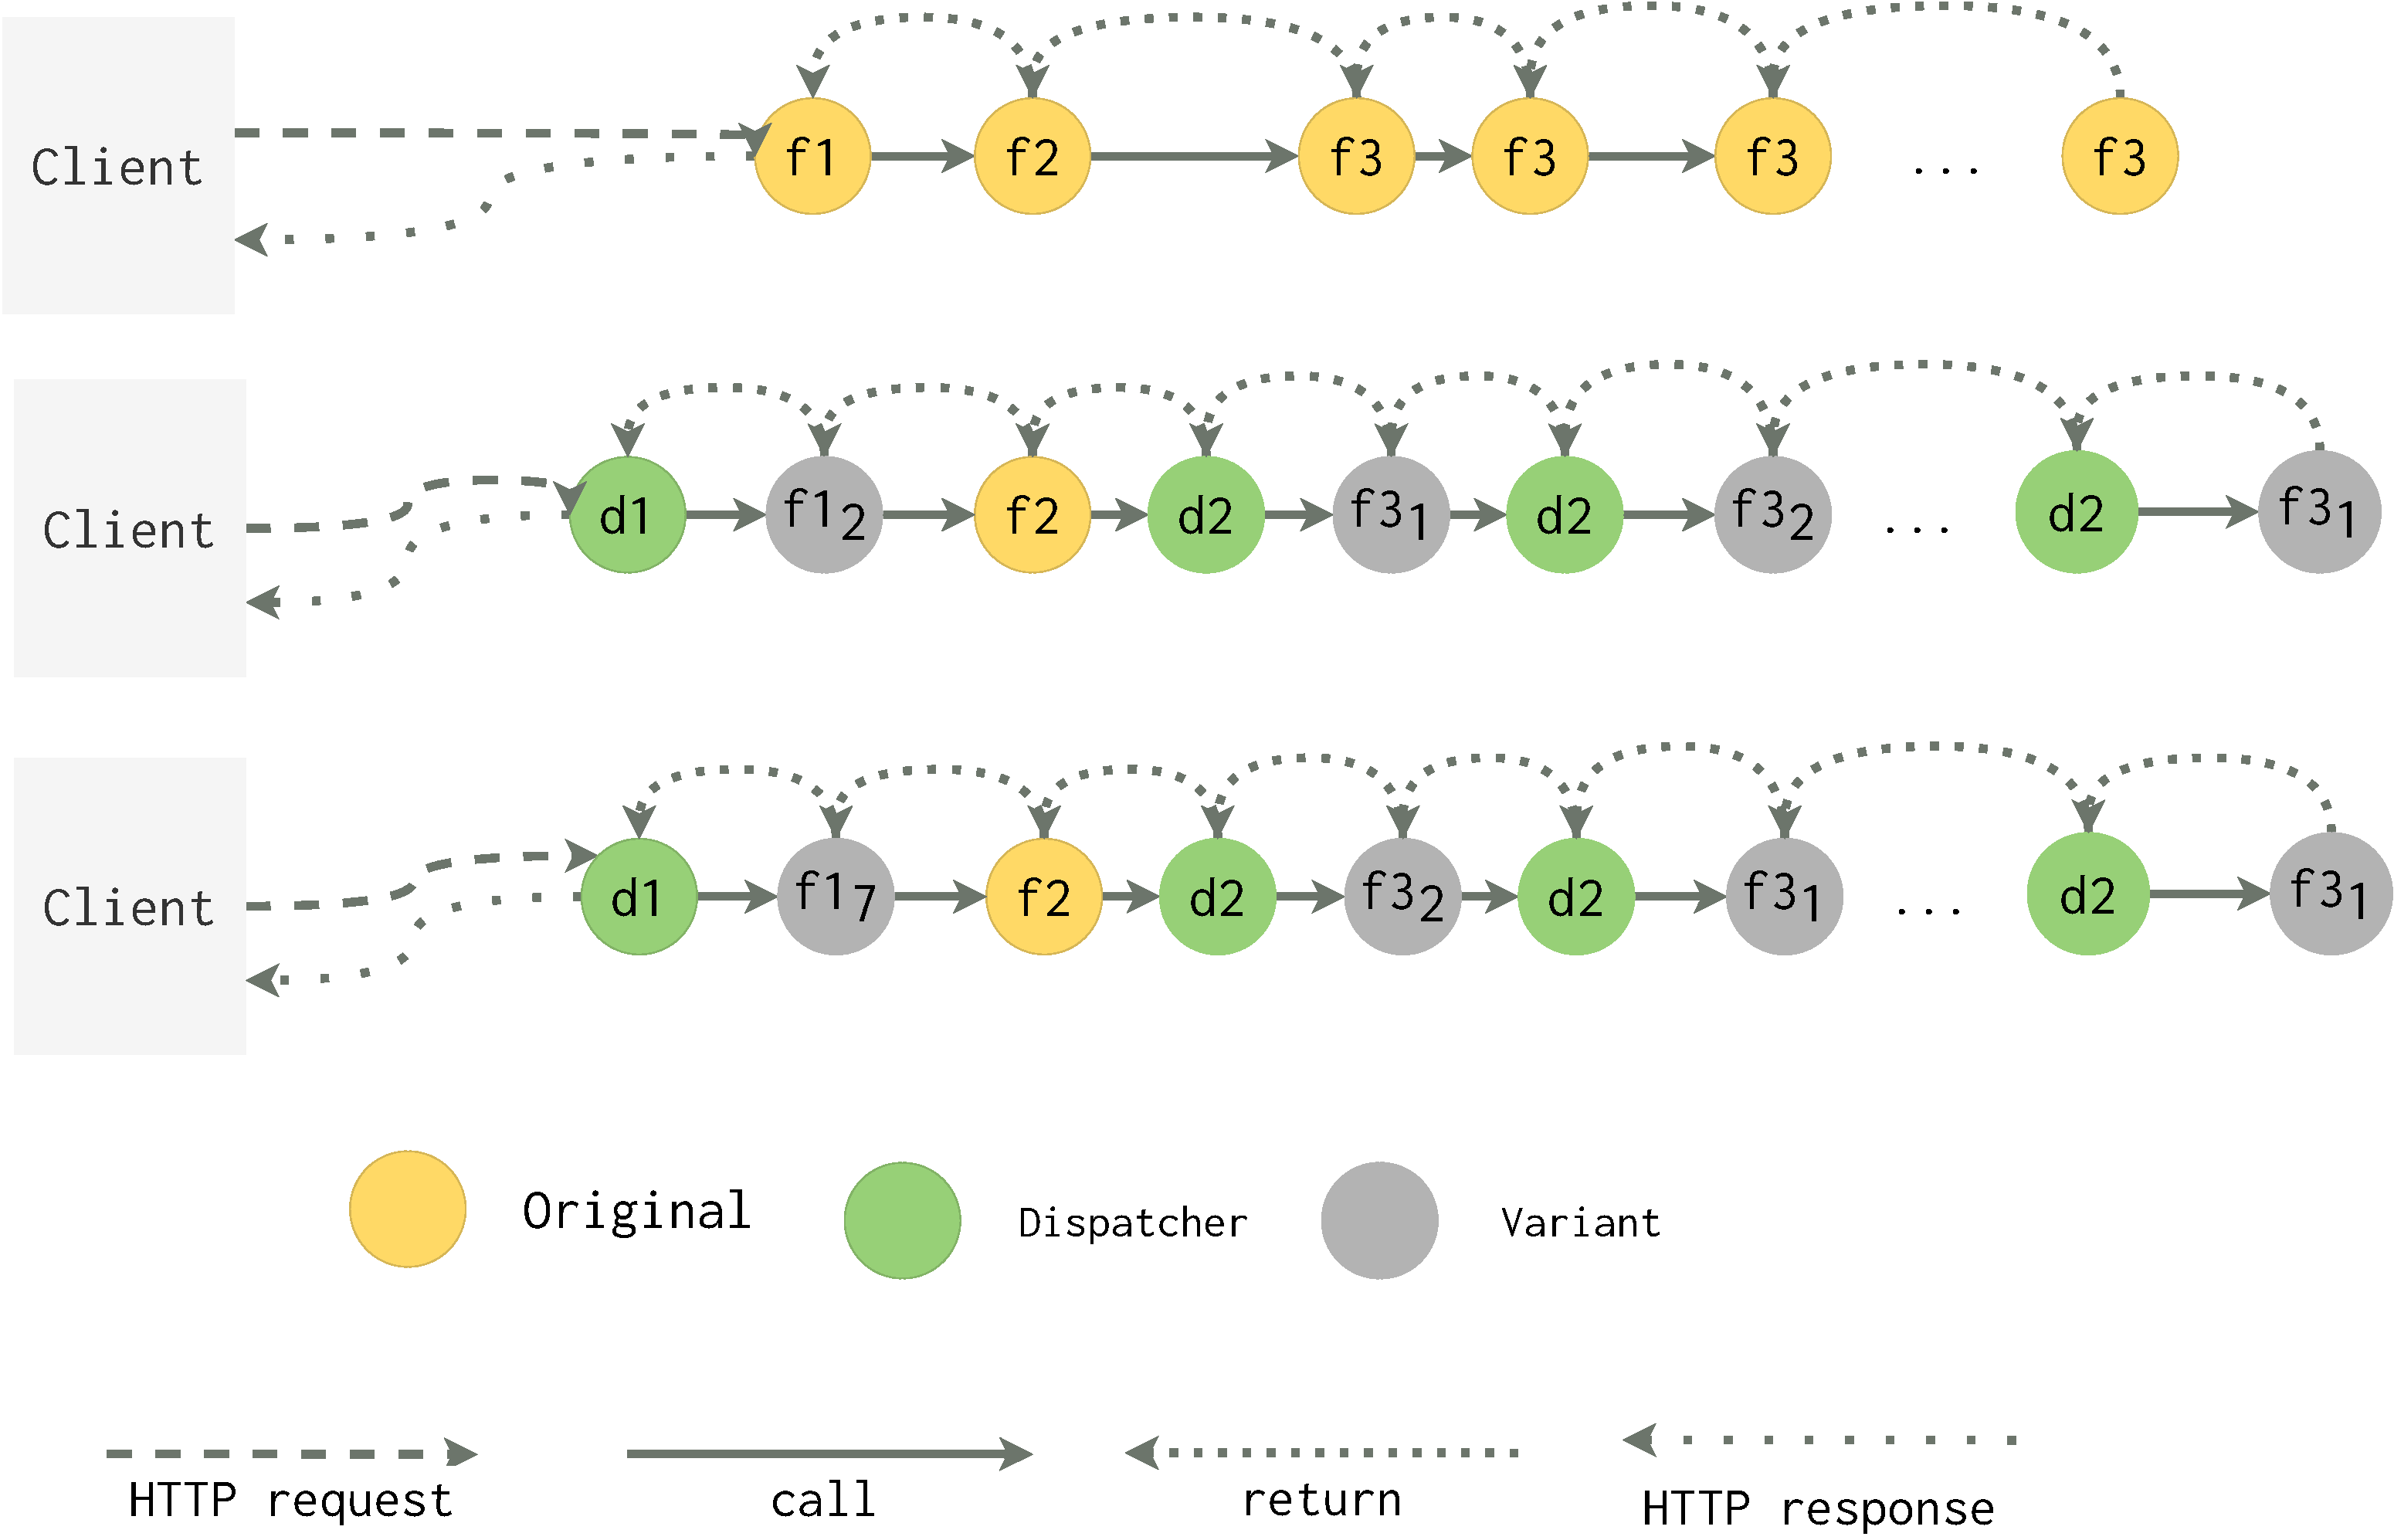
\includegraphics[width=1\linewidth]{diagrams/traces.pdf}
  \caption{Top: an execution trace for the  \texttt{bin2base64} endpoint. Middle and bottom: two different execution traces for the multivariant \texttt{bin2base64}, exhibited by two different requests with exactly the same input.}
  \label{http:workflow}
\end{figure}

% How it works
\autoref{http:workflow} illustrates  the runtime behavior of the original and the multivariant binary,  when deployed on an Edge node.
The top most diagram illustrates the execution trace for the  original of the endpoint \texttt{bin2base64}.
When the HTTP request with the input \texttt{"HelloWorld!"} is received, it invokes functions $f1$, $f2$ followed by 27 recursive calls of function $f3$. Then, the endpoint sends the result \texttt{"0x000xccv0x10x00b3Jsx130x000x00 0x00xpopAHRvdGE="} of its base64 encoding in an HTTP response.

The two diagrams at the bottom of \autoref{http:workflow} illustrate two executions traces observed through two different requests to the endpoint \texttt{bin2base64}.
In the first case, the request first triggers the invocation of dispatcher $d1$, which randomly decides to invoke the variant $f1_2$; then $f2$, which has not been diversified by \tool, is invoked; then the recursive invocations to $f3$ are replaced by iterations over the execution of dispatcher $d2$ followed by a random choice of variants of $f3$. Eventually the result is computed and sent back as an HTTP response. 
The second execution trace of the multivariant binary shows the same sequence of dispatcher and function calls as the previous trace, and also shows that for a different requests, the variants of $f1$ and $f3$ are different. 


The key insights from these figures are as follows. First, from a client's point of view, a request to the original or to a multivariant endpoint, is completely transparent. Clients send the same data, receive the same result, through the same protocol, in both cases.
Second, this figure shows that, at runtime, the execution paths for the same endpoint are different from one execution to another, and that this randomization process results from multiple random choices among function variants, made through the execution of the endpoint.
%From an attacker's perspective, this random selection of variants constantly moves the attack surface and is meant to render a potential vulnerability harder to reach or exploit \cite{davi2015isomeron, 10.5555/3091125.3091155, BEKIROGLU2021106601}.


\end{comment}
